\section{Purpose, System Role, and High-Level Architecture}
\label{sec:purpose}

The Embedded Linux server application is the central software component of the Measurement Network Gateway (MNG) running on the Zynq-based FPGA platform under PetaLinux. Its primary role is to bridge time-sensitive measurements originating from heterogeneous on-board sources (precision temperature sensing, dual ADC acquisition, and digital GPIO inputs) into a deterministic, binary network stream that can be consumed by a remote control computer via Ethernet. In other words, the application constitutes the gateway function: it interacts downward with the FPGA/driver domain to acquire sensor information, and upward with the network domain to provide this information to a TCP client. This role directly aligns with the system-level definition where the MNG acts as a TCP server and the control computer acts as a TCP client (REQ-1), while also satisfying the design constraint that the software is implemented on Embedded Linux (REQ-13) and implemented as a multithreaded program (REQ-14).

From an architectural perspective, the application is structured around two cooperating execution contexts (threads) with clearly separated responsibilities: a sensor acquisition thread that performs periodic sampling and timestamping, and a TCP service thread that handles command/response communication with the remote client. The fundamental design intention behind this separation is to decouple sampling timing from network timing. Network transmission is inherently bursty and client-driven, while sampling must remain stable and predictable. Therefore, a shared ring buffer is introduced as an intermediate storage layer. This buffer is mutex-protected to ensure thread safety, and it is intentionally designed to drop the oldest samples when full, thereby preventing a stalled network from blocking real-time acquisition and keeping the application responsive and stable under overload.

A particularly useful design feature implemented in this server is the ability to run in two distinct modes: a real hardware mode that accesses the measurement kernel driver through \texttt{/dev/meascdd}, and a fake sensor mode that synthetically generates sensor values when the device node is unavailable. This optional functionality significantly improves testability and reproducibility in development environments where the FPGA/driver stack may not be present, and it supports systematic functional verification setups (REQ-26) without requiring full hardware availability.

\subsection{Main Program Entry and Execution Flow (Code Evidence)}
\label{subsec:main-entry}

The program begins by opening the measurement driver device node and selecting the operating mode accordingly. The following excerpt shows the decision point that selects between real and fake acquisition:

\begin{lstlisting}
	fd = open("/dev/meascdd", O_RDWR);
	
	if (fd < 0) {
		perror("open(/dev/meascdd)");
		printf("=> /dev/meascdd not found, running in FAKE SENSOR mode.\n");
		use_fake_sensor = 1;
	} else {
		printf("=> /dev/meascdd opened successfully, REAL HW mode.\n");
		use_fake_sensor = 0;
	}
\end{lstlisting}

The explicit initialization of sample-rate configuration to zero is not accidental: in this implementation, a sampling rate of zero is interpreted as ``disabled'', which realizes the selectable sensors requirement through configuration rather than compile-time switching (REQ-7). The program then remains active until the TCP thread requests shutdown; after that, a controlled termination sequence is executed, including thread joins and resource destruction. This approach provides a clear startup and shutdown procedure (REQ-18), ensures initialization of required resources at startup (REQ-19), and guarantees that threads and allocated resources are properly terminated and destroyed at shutdown (REQ-21).
\subsection{Architecture Diagram}
\label{subsec:architecture-diagram}

\begin{figure}[H]
	\centering
	% Replace with your actual image file
	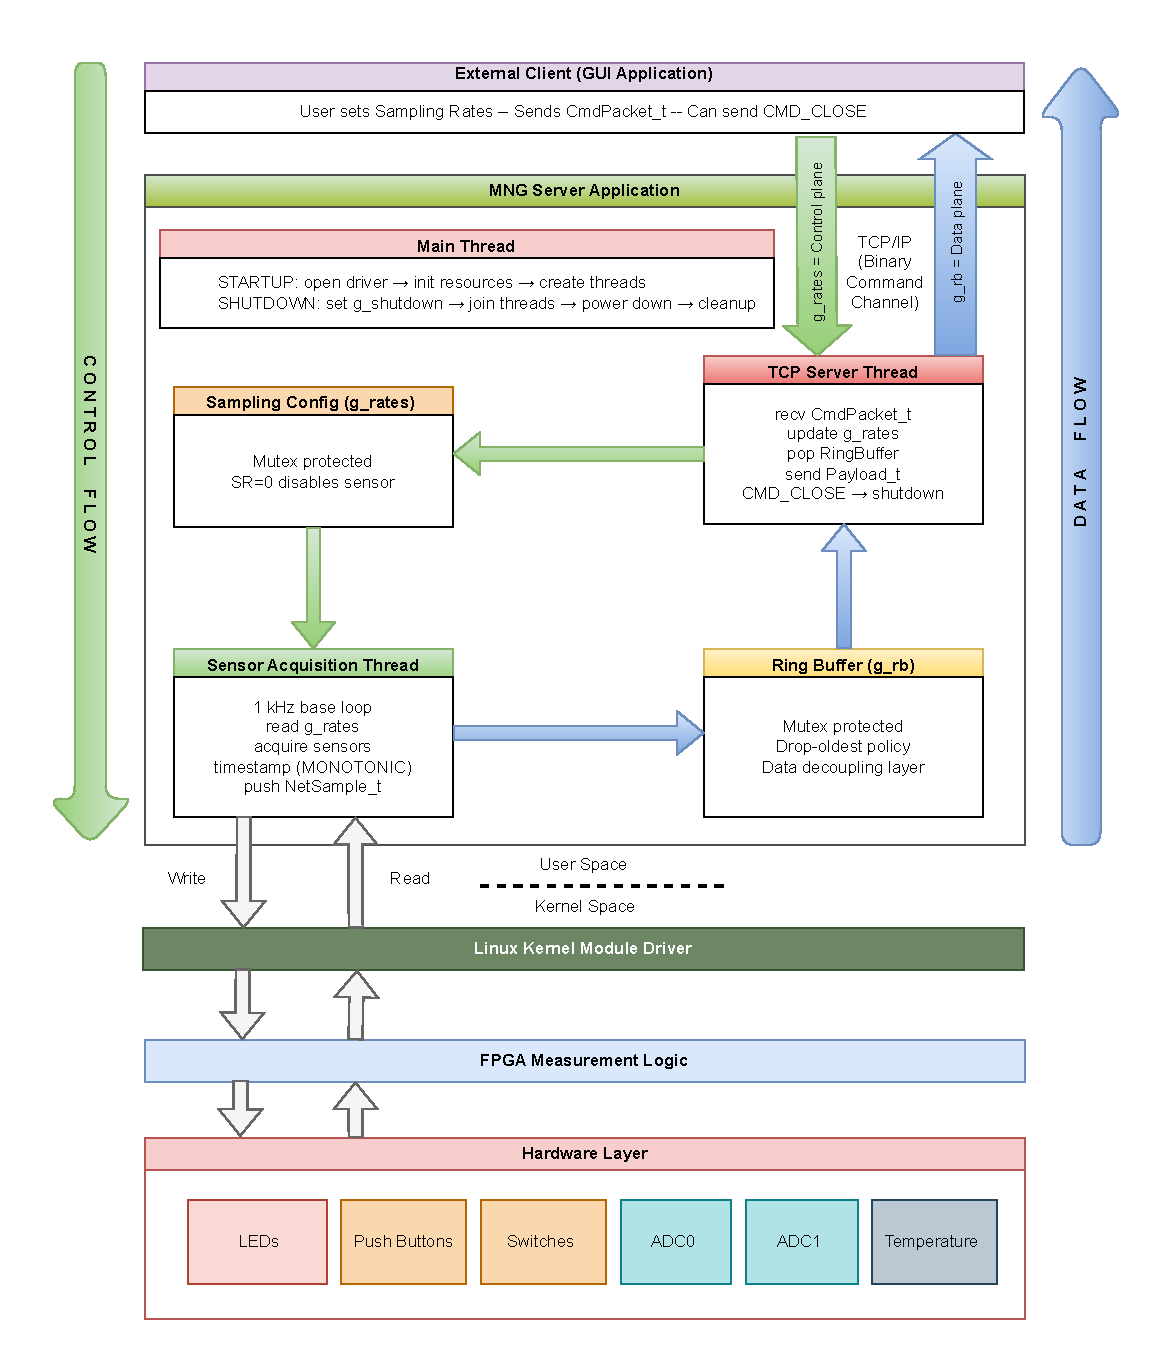
\includegraphics[width=0.9\textwidth]{figures/cmd_get_data_sequence.pdf}
	\caption{Overall software architecture of the Measurement Network Gateway (MNG)}
	\label{fig:mng_architecture}
\end{figure}

Figure~\ref{fig:mng_architecture} illustrates the complete layered architecture of the Measurement Network Gateway (MNG) server system, including the external GUI client, the user-space server application, the Linux kernel driver boundary, the FPGA measurement logic, and the underlying hardware layer. The diagram explicitly distinguishes between the data plane and the control plane, which constitute two orthogonal communication paths within the system.

The data flow propagates upward from the hardware layer toward the external client. Physical measurements originating from temperature sensors, ADC channels, and digital inputs are first processed by the FPGA measurement subsystem and exposed via a register-based interface. The Linux kernel module driver provides a controlled abstraction of this hardware interface through the device node \texttt{/dev/meascdd}. The sensor acquisition thread periodically retrieves measurement values via \texttt{read}/\texttt{write} system calls, timestamps each sample using a monotonic clock source, and pushes the resulting \texttt{NetSample\_t} structures into a mutex-protected ring buffer. The TCP server thread subsequently consumes buffered samples and transmits them to the GUI client using a bounded binary payload.

In contrast, the control flow propagates downward from the GUI client to the acquisition logic. Configuration commands are transmitted via a binary TCP protocol using \texttt{CmdPacket\_t} messages. The TCP thread updates the global sampling-rate configuration structure (\texttt{g\_rates}), which is protected by a mutex to ensure thread-safe concurrent access. The sensor acquisition thread reads this configuration at deterministic cycle boundaries, thereby enabling runtime reconfiguration without interrupting system operation.

A central architectural element is the explicit decoupling between deterministic sampling and asynchronous network communication. The sensor acquisition thread operates at a fixed 1~kHz base rate and derives individual sensor frequencies through integer divisors, thereby maintaining a stable time base. The ring buffer acts as a producer--consumer boundary between acquisition and transmission. By employing a drop-oldest overflow policy, the system ensures that slow or bursty network conditions cannot block time-critical acquisition tasks. This design decision prioritizes temporal consistency and system stability over historical completeness of data, which is appropriate for real-time measurement gateway applications.

The main thread functions exclusively as a lifecycle controller. It performs initialization of shared resources at startup, selects between real hardware mode and synthetic fallback mode, creates worker threads, and supervises cooperative shutdown via a shared termination flag. During shutdown, all threads are joined deterministically, hardware components are powered down where applicable, and all synchronization primitives and file descriptors are released. The clear separation between user space and kernel space, illustrated in the diagram, further emphasizes the layered design philosophy: hardware-specific logic remains encapsulated in the driver layer, while application-level logic operates independently in user space.

Overall, the architecture shown in Figure X.1 demonstrates a structured, modular, and concurrency-aware design that satisfies timing precision, configurability, resource management, and binary protocol efficiency requirements while maintaining clear separation of concerns across all system layers.

\subsection{Protocol and Data Model (Context for Later Sections)}
\label{subsec:protocol-model}

To ensure efficient network transport and compliance with the payload limitation for a single TCP/IP transmission (REQ-17), the server transmits measurements in a strictly binary format (REQ-16). Each measurement is represented as a packed \texttt{NetSample\_t} structure of exactly 14 bytes:

\begin{lstlisting}
	typedef struct __attribute__((packed)) {
		uint64_t time;       // timestamp: microseconds (monotonic)
		uint16_t sensor_id;  // which sensor
		int32_t  value;      // measured value
	} NetSample_t;
	
	#define NETSAMPLE_SIZE 14
\end{lstlisting}

The total size of one sample is therefore:

\[
\text{sizeof(NetSample\_t)} =
8~\text{bytes} + 2~\text{bytes} + 4~\text{bytes}
= 14~\text{bytes}
\]

Each TCP response contains a 32-bit sample counter followed by up to
\( N = 104 \) packed samples:

\begin{lstlisting}
	#define SAMPLES_PER_RESPONSE 104
	
	typedef struct {
		uint32_t count;
		NetSample_t buf[SAMPLES_PER_RESPONSE];
	} Payload_t;
\end{lstlisting}

The maximum payload size is therefore:

\[
\begin{aligned}
	\text{Payload}_{\max}
	&= 4~\text{bytes (count)} + N \cdot 14~\text{bytes} \\
	&= 4 + 104 \cdot 14 \\
	&= 4 + 1456 \\
	&= 1460~\text{bytes}
\end{aligned}
\]

This value is deliberately engineered to remain below the classical
Ethernet MTU constraint of

\[
\text{MTU}_{\text{Ethernet}} = 1500~\text{bytes}
\]

Under standard IPv4/TCP transport, the usable TCP payload per Ethernet frame is:

\[
1500 - 20_{\text{IP header}} - 20_{\text{TCP header}}
= 1460~\text{bytes}
\]

Thus,

\[
\text{Payload}_{\max} = 1460~\text{bytes}
\leq 1500~\text{bytes}
\]

which ensures that each response fits into a single TCP segment under
typical Ethernet conditions, thereby minimizing segmentation overhead
and supporting deterministic transmission behavior.

By using packed binary structures without ASCII conversion or floating-point formatting, the implementation guarantees both compactness and predictable frame sizing, directly satisfying REQ-16 and REQ-17.

\section{Detailed Software Architecture and Concurrency Model}
\label{sec:concurrency}

The internal architecture of the MNG server application is deliberately designed around a strict separation of concerns between time-deterministic sensor acquisition and event-driven network communication. This separation is not merely an implementation detail but a core architectural decision required to satisfy multiple design and RAMS constraints simultaneously. In particular, REQ-14 explicitly requires a multithreaded implementation, while REQ-27 (timing precision and jitter evaluation) implicitly demands that sampling execution must not be blocked or distorted by network delays.

To fulfill these constraints, the application is structured around three concurrent execution contexts:

\begin{itemize}
	\item Main control thread
	\item Sensor acquisition thread
	\item TCP service thread
\end{itemize}

Together, these components form a structured producer--consumer architecture with deterministic timing boundaries.

\begin{figure}[H]
	\centering
	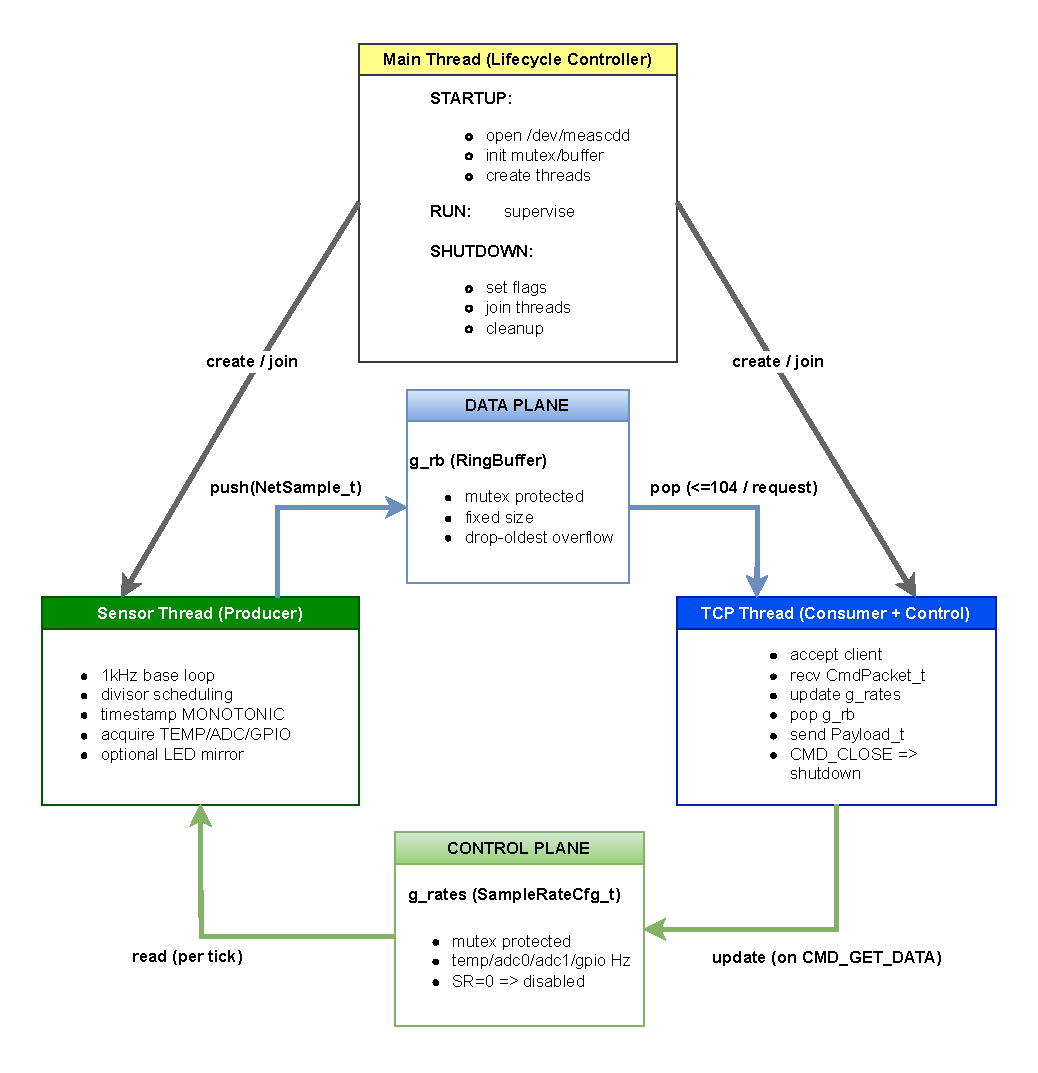
\includegraphics[width=0.95\textwidth]{figures/concurrency_architecture.pdf}
	\caption{Thread interaction model of the MNG server.}
	\label{fig:concurrency-architecture}
\end{figure}
Figure~\ref{fig:concurrency-architecture} illustrates the complete runtime interaction model of the server application. The main thread acts as a lifecycle controller responsible for initialization, supervision, and coordinated shutdown. It creates and joins both worker threads while remaining logically separated from real-time acquisition and network communication responsibilities.

The sensor thread operates as the deterministic producer within the data plane. It executes a fixed 1~kHz base loop, performs divisor-based scheduling, timestamps measurements using a monotonic clock, and pushes \texttt{NetSample\_t} objects into the mutex-protected ring buffer (\texttt{g\_rb}). The ring buffer constitutes the producer--consumer boundary and ensures that acquisition timing remains independent of network conditions.

The TCP thread acts simultaneously as consumer and control interface. It pops buffered samples (up to 104 per request), packages them into a bounded payload, and transmits them over TCP. Additionally, it updates the shared configuration structure (\texttt{g\_rates}) upon receiving \texttt{CMD\_GET\_DATA} commands. This configuration structure forms the control plane and is accessed atomically by both threads via mutex protection.

The explicit separation between data plane and control plane guarantees that configuration updates do not interfere with deterministic sampling. Likewise, the drop-oldest overflow policy prevents network delays from blocking acquisition. The diagram therefore visualizes the architectural principles of concurrency separation, bounded buffering, and cooperative lifecycle control that define the server design.

\subsection{Thread Lifecycle and Responsibility Separation}
\label{subsec:thread-lifecycle}

The \texttt{main()} function serves exclusively as a system orchestrator. It initializes global resources, creates both worker threads, supervises shutdown signaling, and performs deterministic cleanup at termination. Importantly, the main thread itself does not perform sampling nor network communication; this prevents unintended coupling between initialization logic and runtime processing.

Thread creation is realized using POSIX threads:

\begin{lstlisting}
	if (pthread_create(&sensor_th, NULL, sensor_thread, &scfg) != 0) {
		perror("pthread_create(sensor)");
	}
	
	if (pthread_create(&tcp_th, NULL, tcp_thread, NULL) != 0) {
		perror("pthread_create(tcp)");
	}
\end{lstlisting}

The choice of separate threads ensures that blocking socket operations cannot introduce jitter into the deterministic sampling loop.

Shutdown coordination is implemented via a global flag:

\begin{lstlisting}
	static volatile int g_shutdown = 0;
\end{lstlisting}

Both worker threads periodically evaluate this flag and terminate cooperatively. This design avoids abrupt cancellation and satisfies REQ-21.

\subsection{Producer--Consumer Decoupling via Ring Buffer}

A central architectural element of the system is the ring buffer implementation. The ring buffer decouples the deterministic sampling process from the asynchronous network transmission. Its structure is defined as:

\begin{lstlisting}[language=C]
	typedef struct {
		
		pthread_mutex_t mutex;
		
		NetSample_t     buf[RBUF_LEN];
		
		int             head;   // write index
		
		int             tail;   // read index
		
		int             count;  // number of stored elements
		
	} RingBuffer_t;
\end{lstlisting}

The buffer size is fixed at:

\begin{lstlisting}[language=C]
	#define RBUF_LEN 312
\end{lstlisting}

The decision to use a fixed-size circular buffer instead of dynamic allocation is intentional. In embedded Linux environments, predictable memory behavior is preferred over dynamic allocation at runtime, particularly in long-running processes. This avoids heap fragmentation and aligns with RAMS considerations regarding system stability.

The push operation demonstrates a deliberate overflow policy:

\begin{lstlisting}[language=C]
	if (rb->count == RBUF_LEN) {
		
		rb->tail = (rb->tail + 1) % RBUF_LEN;  // drop oldest
		
	} else {
		
		rb->count++;
		
	}
\end{lstlisting}

Instead of blocking when the buffer is full, the system discards the oldest sample. This policy ensures that the sampling thread never blocks due to slow network consumption. From a systems perspective, this choice prioritizes real-time acquisition continuity over historical completeness. In measurement gateway applications, maintaining current data flow is often more critical than preserving outdated samples.

The pop operation is non-blocking:

\begin{lstlisting}[language=C]
	if (rb->count == 0) {
		
		pthread_mutex_unlock(&rb->mutex);
		
		return 0;
		
	}
\end{lstlisting}

This design prevents the TCP thread from blocking indefinitely when no data is available. Instead, it simply returns zero samples, and the client receives an empty response. This behavior maintains responsiveness and supports REQ-26 (testability) by allowing observation of system behavior even under idle conditions.

\subsection{Timing Strategy and Deterministic Sampling}

One of the most important architectural aspects of the server is its deterministic timing model. The sensor thread operates on a fixed base loop frequency:

\begin{lstlisting}[language=C]
	#define BASE_RATE_HZ 1000u
\end{lstlisting}

This defines a 1 kHz base sampling tick (1 ms period). Instead of running each sensor independently, all sensor activities are derived from this base tick using integer divisors:

\begin{lstlisting}[language=C]
	uint32_t temp_div = (temp_hz > 0) ? (BASE_RATE_HZ / temp_hz) : 0;
\end{lstlisting}

This design has several advantages:

\begin{itemize}
	\item All sampling operations are synchronized to a common time base.
	\item Sampling frequency changes can be applied dynamically.
	\item Relative timing between sensors remains deterministic.
\end{itemize}

The base loop delay is implemented using \texttt{nanosleep}:

\begin{lstlisting}[language=C]
	struct timespec req;
	
	req.tv_sec  = 0;
	
	req.tv_nsec = 1 * 1000000L;  // 1 ms
	
	nanosleep(&req, NULL);
\end{lstlisting}

While \texttt{nanosleep} does not provide hard real-time guarantees under standard Linux scheduling, it is sufficient for soft real-time measurement applications in Embedded Linux environments. Furthermore, jitter can be evaluated using timestamps (REQ-27).

\subsection{Timestamping and Temporal Consistency}

Every measurement is timestamped using the monotonic clock:

\begin{lstlisting}[language=C]
	static uint64_t get_time_us(void)
	{
		struct timespec ts;
		
		clock_gettime(CLOCK_MONOTONIC, &ts);
		
		return (uint64_t)ts.tv_sec * 1000000ull + ts.tv_nsec / 1000ull;
	}
\end{lstlisting}

The use of CLOCK MONOTONIC instead of CLOCK REALTIME is a deliberate design decision. Real-time clocks may be adjusted by the system (e.g., NTP synchronization), which would introduce discontinuities in measurement time. In contrast, the monotonic clock guarantees strictly increasing timestamps independent of wall-clock corrections. This ensures temporal consistency and supports accurate delay and jitter evaluation (REQ-27).

The timestamp is stored directly inside each transmitted sample:

\begin{lstlisting}[language=C]
	pkt.time = time;
\end{lstlisting}

Thus, every measurement is self-contained and temporally traceable, fully satisfying REQ-8.

\subsection{Sample Rate Configuration Mechanism}

Sampling rates are stored in a mutex-protected global configuration structure:

\begin{lstlisting}[language=C]
	typedef struct {
		
		pthread_mutex_t mutex;
		
		uint32_t temp_hz;
		
		uint32_t adc0_hz;
		
		uint32_t adc1_hz;
		
		uint32_t gpio_hz;
		
	} SampleRateCfg_t;
\end{lstlisting}

This design allows dynamic reconfiguration without restarting the application. The TCP thread updates the configuration when receiving a \texttt{CMD\_GET\_DATA} packet:

\begin{lstlisting}[language=C]
	pthread_mutex_lock(&g_rates.mutex);
	
	g_rates.temp_hz = sr_temp;
	
	g_rates.adc0_hz = sr_adc0;
	
	g_rates.adc1_hz = sr_adc1;
	
	g_rates.gpio_hz = sr_gpio;
	
	pthread_mutex_unlock(&g_rates.mutex);
\end{lstlisting}

The sensor thread reads the configuration atomically at each base tick. This ensures that configuration changes are applied deterministically at the next cycle boundary.

A sample rate of zero is interpreted as disabled:

\begin{lstlisting}[language=C]
	uint32_t temp_div = (temp_hz > 0) ? (BASE_RATE_HZ / temp_hz) : 0;
\end{lstlisting}

This implementation satisfies:

\begin{itemize}
	\item REQ-6 (configurable sampling rate per signal)
	\item REQ-7 (selectable sensors)
	\item REQ-9 and REQ-10 (configuration via control program)
\end{itemize}

\section{Hardware Interaction Layer and Kernel Driver Communication}

The hardware interaction layer of the MNG server represents the boundary between user-space software and FPGA-based measurement logic. This layer is responsible for translating high-level measurement requests into register-level transactions via the Linux kernel driver (/dev/meascdd). It is implemented entirely in user space but relies on a structured data exchange mechanism \texttt{MeasObj\_struct} that abstracts register-based communication with the FPGA subsystem.

This architectural separation ensures that hardware-specific access logic remains encapsulated within the kernel module, while the server application operates at a higher abstraction level. Such layering improves portability, modularity, and maintainability, and it aligns with good embedded Linux design practice.

\subsection{Driver Interface and Register Transaction Model}

Communication with the FPGA measurement subsystem is performed using the following structure:

\begin{lstlisting}[language=C]
	typedef struct {
		
		unsigned int rnum;
		
		unsigned int rvalue;
		
	} MeasObj_struct;
\end{lstlisting}

Each transaction consists of:

\begin{itemize}
	\item A register number (rnum)
	\item A register value (rvalue)
\end{itemize}

Data exchange is performed using standard write() and read() system calls on the device node:

\begin{lstlisting}[language=C]
	ret = write(fd, &TF_Obj_Snd, MEASOBJ_SIZE);
	
	ret = read(fd, &TF_Obj_Rcv, MEASOBJ_SIZE);
\end{lstlisting}

This approach satisfies REQ-13 (Embedded Linux) by using standard POSIX system calls rather than custom kernel hooks. It also ensures binary communication without ASCII conversion (REQ-16).

The constant:

\begin{lstlisting}[language=C]
	#define REGNUM_ID 0x0FF
\end{lstlisting}

is used as a polling register identifier to query hardware status flags. The driver-level polling loop in MaxRead() demonstrates a synchronous register transaction model:

\begin{lstlisting}[language=C]
	do {
		
		TF_Obj_Snd.rnum   = REGNUM_ID;
		
		TF_Obj_Snd.rvalue = 1;
		
		write(fd, &TF_Obj_Snd, MEASOBJ_SIZE);
		
		read(fd, &TF_Obj_Rcv, MEASOBJ_SIZE);
		
		xdata = TF_Obj_Rcv.rvalue;
		
	} while (((xdata & 0x01) == 0) && (k < 1000));
\end{lstlisting}

The loop waits until a hardware-ready flag becomes set or a timeout occurs. This polling-based approach simplifies synchronization and avoids interrupt-driven complexity in user space.

\subsection{Temperature Acquisition (MAX31865 – REQ-2)}

Temperature measurement is performed using a precision resistive temperature sensor connected through a MAX31865 interface. The acquisition process includes:

\begin{itemize}
	\item Power-up and initialization
	\item Conversion start
	\item Status polling
	\item MSB/LSB register read
	\item 15-bit raw value extraction
\end{itemize}

Initialization sequence:

\begin{lstlisting}[language=C]
	static void PMB1_Init(int fd)
	{
		TF_Obj_Snd.rnum   = 0;
		
		TF_Obj_Snd.rvalue = 0x022;
		
		write(fd, &TF_Obj_Snd, MEASOBJ_SIZE);
		
		MaxWrite(fd, 0x00, 0x081);   // power up MAX31865
	}
\end{lstlisting}

Conversion start:

\begin{lstlisting}[language=C]
	MaxWrite(fd, 0x00, 0x0a1);  // start conversion
\end{lstlisting}

Data readout:

\begin{lstlisting}[language=C]
	xdata = MaxRead(fd, 0x01);   // MSB
	
	xdata <<= 8;
	
	xlsb  = MaxRead(fd, 0x02);   // LSB
	
	xdata |= (xlsb & 0xff);
	
	xadc = xdata >> 1;
\end{lstlisting}

The raw ADC value is intentionally transmitted without floating-point conversion. This design decision preserves precision and ensures that no ASCII or float formatting is performed before network transmission (REQ-16). Temperature conversion to physical units can be performed on the client side if required.

Power-down is explicitly handled during shutdown:

\begin{lstlisting}[language=C]
	MaxWrite(cfg->fd, 0x00, 0x001); // power down PMB1
\end{lstlisting}

This fulfills REQ-20 (disable sensors on termination).

\subsection{ADC Acquisition (REQ-3)}

The system captures data from two ADC channels via a PmodAD1 module. Both channels are acquired simultaneously in a single 32-bit word:

\begin{lstlisting}[language=C]
	*adc0 = (uint16_t)(adc_word & 0x0fff);
	
	*adc1 = (uint16_t)((adc_word >> 16) & 0x0fff);
\end{lstlisting}

Each channel is 12-bit wide. The server keeps the channels logically separated using different \texttt{sensor\_id} values:

\begin{lstlisting}[language=C]
	#define SENSOR_ID_ADC0 2
	
	#define SENSOR_ID_ADC1 3
\end{lstlisting}

Although acquisition is simultaneous at hardware level, transmission is decoupled logically. Each ADC channel is treated as an independent sensor stream, enabling independent sampling rate configuration (REQ-6).

\subsection{Digital Inputs: Switches and Pushbuttons (REQ-4, REQ-5)}

Digital input acquisition is performed via register 0:

\begin{lstlisting}[language=C]
	*switches = (uint8_t)(val & 0xff);
	
	*pushb    = (uint8_t)((val >> 8) & 0x1f);
\end{lstlisting}

The design combines both into a single logical sensor group:

\begin{lstlisting}[language=C]
	pkt.sensor_id = SENSOR_ID_GPIO;
	
	pkt.value = ((int32_t)pb_state << 8) | (int32_t)sw_state;
\end{lstlisting}

This compact encoding reduces payload size and ensures efficient transmission. It also satisfies REQ-25, which specifies that switches and push buttons shall be used as auxiliary digital input signals.

\subsection{LED Mirror Feature (Optional Enhancement)}

An additional feature implemented in the sensor thread mirrors switch states to onboard LEDs:

\begin{lstlisting}[language=C]
	Write_LEDs(cfg->fd, sw_state);
\end{lstlisting}

This functionality is not explicitly required in the requirements specification but represents a valuable diagnostic feature. It provides immediate visual feedback that confirms correct GPIO readout and driver interaction. Such features improve testability and development efficiency, especially in early integration phases.

\subsection{Fake Sensor Mode (Design Enhancement)}

If /dev/meascdd cannot be opened, the system automatically switches to a synthetic signal generator mode:

\begin{lstlisting}[language=C]
	if (fd < 0) {
		
		use_fake_sensor = 1;
		
	}
\end{lstlisting}

In fake mode:

\begin{itemize}
	\item ADC values are generated as sine waves
	\item Temperature increases incrementally
	\item GPIO values default to zero
\end{itemize}

Example sine generation:

\begin{lstlisting}[language=C]
	double v0 = offset + amp * sin(2.0 * M_PI * 2.0 * t);
\end{lstlisting}

This feature is particularly valuable for:

\begin{itemize}
	\item Offline GUI development
	\item Network testing without hardware
	\item Timing analysis under controlled conditions
\end{itemize}

Although not explicitly required, this functionality strongly supports REQ-26 (functional testing).

\section{TCP Communication Protocol and Binary Payload Design}

The network communication layer of the MNG server is implemented as a TCP/IP service that exposes measurement data to a remote control computer. The design adopts a command/response paradigm rather than a continuous streaming paradigm. This decision is motivated by the need for explicit control over which sensors are active and at what rates they are sampled, as well as by the requirement to keep each TCP transmission within a fixed maximum payload size. In the overall system, the MNG acts as a TCP server while the control computer acts as the TCP client (REQ-1). Consequently, network interaction is initiated by the client, which sends configuration commands and requests data, while the server responds with a bounded set of measurements collected since the last request.

Two goals dominate the protocol design: first, all data exchange must occur in strictly binary form to avoid conversion overhead and preserve compactness (REQ-16). Second, each response must be designed such that it fits into a single Ethernet frame whenever possible, thereby complying with the maximum payload constraint of 1500 bytes (REQ-17) and improving performance by avoiding fragmentation and unnecessary protocol overhead. The implementation explicitly targets approximately one TCP segment worth of data per request.

\subsection{Server Socket Setup and Connection Lifecycle}

The server binds to a fixed TCP port and waits for a single client connection. The socket setup is conventional but deliberately configured for robust restart behavior via \texttt{SO\_REUSEADDR}, which prevents “address already in use” errors after an abnormal termination or a fast restart during development:

\begin{lstlisting}[language=C]
	srv_fd = socket(AF_INET, SOCK_STREAM, 0);
	
	int opt = 1;
	
	setsockopt(srv_fd, SOL_SOCKET, SO_REUSEADDR, &opt, sizeof(opt));
	
	addr.sin_family      = AF_INET;
	
	addr.sin_addr.s_addr = htonl(INADDR_ANY);
	
	addr.sin_port        = htons(TCP_PORT);
	
	bind(srv_fd, (struct sockaddr *)&addr, sizeof(addr));
	
	listen(srv_fd, 1);
	
	cli_fd = accept(srv_fd, (struct sockaddr *)&cli_addr, &cli_len);
\end{lstlisting}

The design uses a single connection model (listen backlog of 1), which is sufficient for the intended laboratory and demonstration scenario where a single control computer interacts with the MNG at a time. Importantly, if the client disconnects or requests termination, the server transitions into a controlled shutdown sequence. This behavior is consistent with RAMS expectations because it avoids leaving worker threads running in an undefined state.

Client disconnect detection is handled via recv() returning 0 bytes, which is the standard TCP indication of an orderly shutdown by the peer:

\begin{lstlisting}[language=C]
	ssize_t n = recv(cli_fd, &cmd, sizeof(cmd), MSG_WAITALL);
	
	if (n == 0) {
		
		printf("[tcp] client closed connection.\n");
		
		g_shutdown = 1;
		
		break;
		
	}
\end{lstlisting}

The same shutdown flag is also set on error conditions, ensuring that network failures lead to a predictable and safe termination path rather than undefined behavior.

\subsection{Command Packet Format and Semantic Meaning}

Figure~\ref{fig:cmd_get_data_sequence} illustrates the complete interaction sequence between the GUI client, the TCP server thread, the sensor thread, the shared ring buffer, and the kernel driver during a \texttt{CMD\_GET\_DATA} request/response cycle.

\begin{figure}[H]
	\centering
	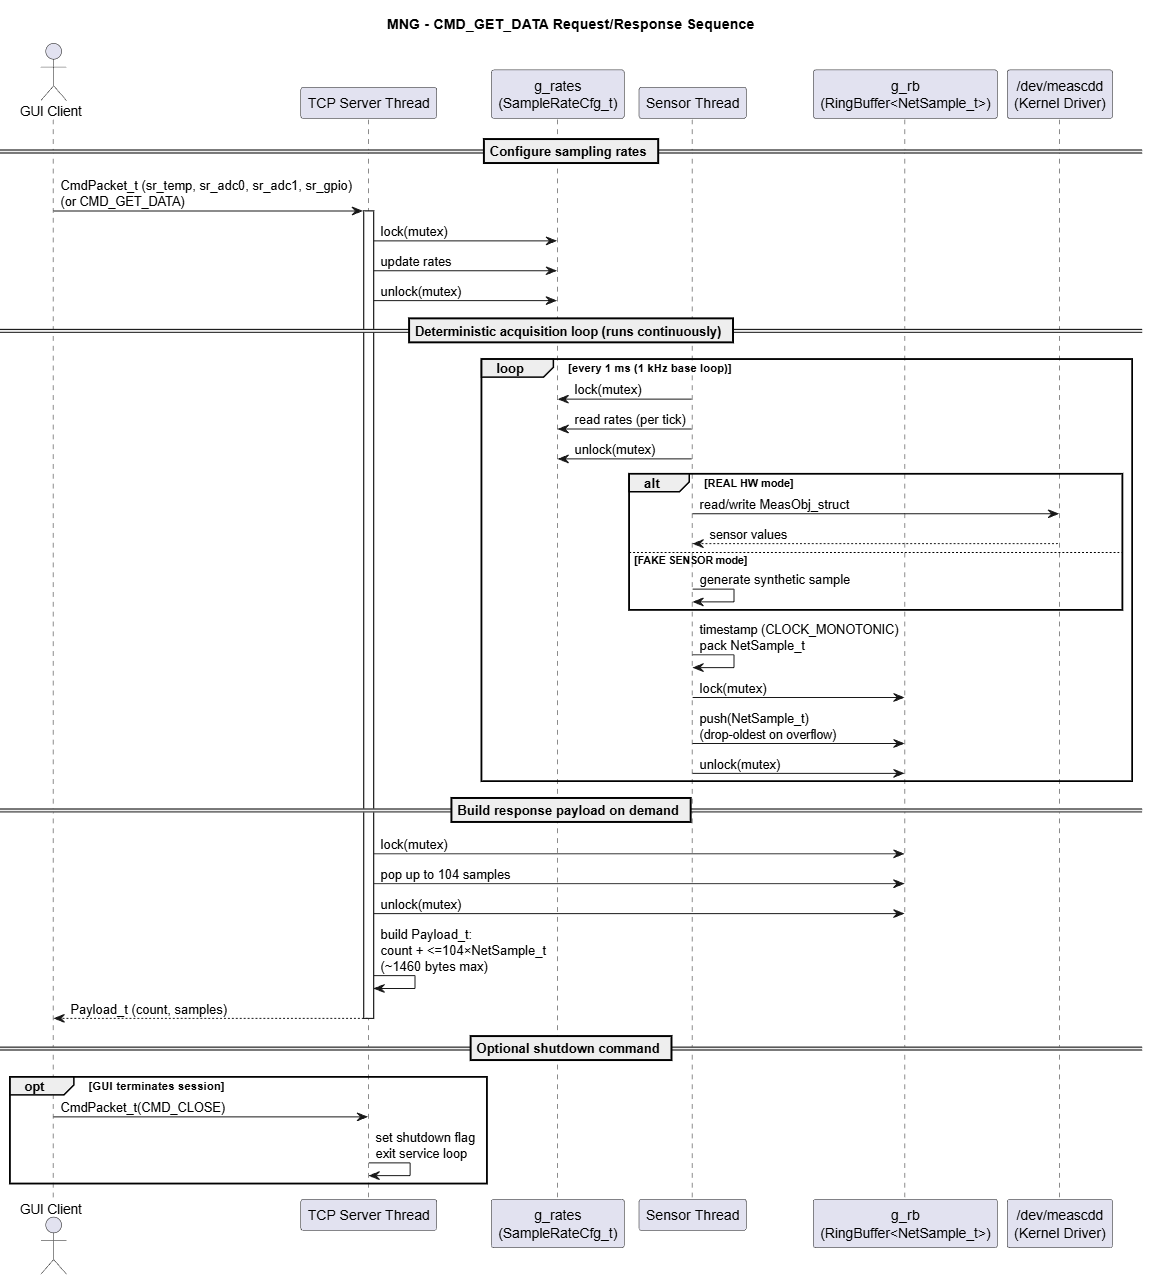
\includegraphics[width=\textwidth]{figures/cmd_get_data_sequence.png}
	\caption{UML Sequence Diagram of the CMD\_GET\_DATA Request/Response Cycle}
	\label{fig:cmd_get_data_sequence}
\end{figure}

The client interacts with the server by sending a fixed-size command structure, \texttt{CmdPacket\_t}, which is explicitly designed as a binary control message:

\begin{lstlisting}[language=C]
	typedef struct __attribute__((packed)) {
		
		uint32_t cmd;      // command code
		
		uint32_t sr_temp;  // TEMP sample rate (Hz)
		
		uint32_t sr_adc0;  // ADC0 sample rate (Hz)
		
		uint32_t sr_adc1;  // ADC1 sample rate (Hz)
		
		uint32_t sr_gpio;  // GPIO sample rate (Hz)
		
	} CmdPacket_t;         // 20 bytes
\end{lstlisting}

Two command codes are implemented:

\begin{lstlisting}[language=C]
	#define CMD_GET_DATA 1
	
	#define CMD_CLOSE    2
\end{lstlisting}

From a protocol perspective, \texttt{CMD\_GET\_DATA} serves a dual purpose. First, it carries the client’s desired sampling rates for each sensor. Second, it acts as a “data request trigger,” instructing the server to respond immediately with a bounded set of samples currently available in the ring buffer. This coupling of configuration and request into a single packet keeps the protocol minimal and avoids extra message exchanges, which further reduces overhead.

The \texttt{CMD\_CLOSE} command enables controlled shutdown initiated by the client. This command is important for meeting REQ-18 and REQ-21 because it ensures the application can terminate cleanly under software control without relying on abrupt termination (e.g., forced kill).

\subsection{Dynamic Reconfiguration of Sampling Rates (Cross-Layer Interaction)}

Upon receiving a \texttt{CMD\_GET\_DATA} request, the TCP thread updates the global sampling-rate configuration. Because the sensor thread reads these rates continuously, a mutex is used to guarantee consistent updates:

\begin{lstlisting}[language=C]
	pthread_mutex_lock(&g_rates.mutex);
	
	g_rates.temp_hz = sr_temp;
	
	g_rates.adc0_hz = sr_adc0;
	
	g_rates.adc1_hz = sr_adc1;
	
	g_rates.gpio_hz = sr_gpio;
	
	pthread_mutex_unlock(&g_rates.mutex);
\end{lstlisting}

This mechanism realizes a runtime reconfiguration capability: a remote client can enable or disable sensors and adjust their sampling frequencies on-the-fly without restarting the server. A sampling rate of zero is interpreted as ``disabled,'' which effectively implements sensor selectability (REQ-7) and sampling rate configurability (REQ-6) using the same configuration path. In the larger system context, the GUI will act as this control client (REQ-9, REQ-10), while the terminal-based test client provides an additional verification path (REQ-26).

\subsection{Response Payload Format and Size Engineering}

The server responds using a payload container that begins with a 32-bit count field followed by count packed samples:

\begin{lstlisting}[language=C]
	typedef struct {
		
		uint32_t   count;
		
		NetSample_t buf[SAMPLES_PER_RESPONSE];
		
	} Payload_t;
\end{lstlisting}

Each sample is defined as a packed 14-byte structure:

\begin{lstlisting}[language=C]
	typedef struct __attribute__((packed)) {
		
		uint64_t time;
		
		uint16_t sensor_id;
		
		int32_t  value;
		
	} NetSample_t;
\end{lstlisting}

\begin{lstlisting}[language=C]
	#define NETSAMPLE_SIZE 14
\end{lstlisting}

The constant \texttt{SAMPLES\_PER\_RESPONSE} is set to 104:

\begin{lstlisting}[language=C]
	#define SAMPLES_PER_RESPONSE 104
\end{lstlisting}

The choice of 104 is not arbitrary. The payload is engineered so that the maximum transmitted size remains below the classical Ethernet MTU threshold. Specifically, the payload size is:

\begin{itemize}
	\item 4 bytes for \texttt{count}
	\item 104 × 14 = 1456 bytes for samples
	\item Total = 1460 bytes
\end{itemize}

This explicitly meets the design requirement that the payload for a single TCP/IP transmission is limited to 1500 bytes (REQ-17). Additionally, by using packed binary structures without ASCII conversion, it satisfies REQ-16.

This is also reflected in the comment embedded in the header:

\begin{lstlisting}[language=C]
	#define SAMPLES_PER_RESPONSE  104   // 4 + 104 * 14 = 1460 bytes (~one TCP segment)
\end{lstlisting}

Packet inspection using Wireshark confirmed that transmitted TCP segments remained below the Ethernet MTU and no IP fragmentation occurred during testing.

From a performance perspective, keeping the payload close to (but below) the typical MTU improves efficiency because it tends to be transmitted as a single TCP segment with minimal fragmentation. While TCP segmentation and IP fragmentation are handled by the stack, avoiding them is beneficial for deterministic timing behavior and overall throughput, particularly in embedded systems where CPU budget and memory copies are non-trivial.

\subsection{Response Generation Logic and Ring Buffer Consumption}

When a \texttt{CMD\_GET\_DATA} is received, the TCP thread attempts to pop up to 104 samples from the ring buffer. The server does not block waiting for data; instead, it returns what is immediately available. This design choice ensures that the client’s request/response cycle remains bounded in time, which is important when the control program (GUI) is expected to refresh live data at interactive rates.

The pop and response filling logic is implemented as:

\begin{lstlisting}[language=C]
	for (int i = 0; i < SAMPLES_PER_RESPONSE; ++i) {
		
		NetSample_t pkt;
		
		if (RingBuffer_pop(&g_rb, &pkt)) {
			g_pl.buf[i] = pkt;
			g_pl.count = g_pl.count + 1;
		} else {
			break;
		}
	}
\end{lstlisting}

If no samples are available, the server sends only the count field (which is zero). This is a deliberate micro-optimization: it avoids sending a full payload with meaningless data and clearly indicates an “empty response” to the client:

\begin{lstlisting}[language=C]
	if (g_pl.count == 0) {
		send(cli_fd, &g_pl.count, sizeof(uint32_t), 0);
	} else {
		send(cli_fd, &g_pl, (sizeof(uint32_t) + (g_pl.count * NETSAMPLE_SIZE)), 0);
	}
	
	g_pl.count = 0;
\end{lstlisting}

A noteworthy point in the implementation is the dummy samples. During development the system considered an alternative strategy where responses could always contain a fixed number of samples by padding with “dummy” entries when the ring buffer is empty. Ultimately, the implemented approach of variable-length responses is more bandwidth-efficient and semantically cleaner, because the client can directly interpret \texttt{count = 0} as “no data available.”

\subsection{Protocol Characteristics: Determinism, Efficiency, and Extensibility}

The implemented protocol exhibits three important characteristics. First, it is deterministic in the sense that response size is bounded and command processing remains lightweight, which reduces jitter induced by network handling. Second, it is efficient: by avoiding ASCII conversions and by sizing responses to fit into a single near-MTU payload, CPU overhead and network overhead are minimized. Third, it remains extensible: additional sensors or additional commands could be introduced by extending the \texttt{sensor\_id} namespace and adding new command codes, while keeping backward compatibility as long as structure sizes and packing rules are preserved.

One subtle but relevant engineering aspect is endianness: because both client and server are intended to run on common little-endian architectures in the lab environment, the code currently sends packed structs without explicit htonl() conversion for fields inside the payload. In a broader deployment scenario with heterogeneous architectures, it would be advisable to define a canonical network byte order for all multi-byte fields to ensure portability. For the intended scope of this project (embedded board + PC), the direct binary transfer is a valid and pragmatic performance optimization aligned with REQ-16.

\section{Startup/Shutdown Procedures, RAMS Compliance, and Resource Management}

A robust embedded measurement gateway must not only deliver correct functional behavior but also provide deterministic startup and shutdown procedures, ensuring that the system can be brought into operation reliably and terminated without leaving the hardware in an undefined state or the software in a resource-leaking condition. In the context of this project, these concerns are formalized in the RAMS requirements (REQ-18 to REQ-21). The MNG server application implements an explicit lifecycle model covering (i) initialization of all required resources at startup, (ii) cooperative termination across threads, (iii) sensor deactivation at shutdown, and (iv) destruction of allocated resources prior to process exit.

The central design principle behind the implemented lifecycle is cooperative shutdown: instead of abruptly cancelling threads or relying on external process termination, a global shutdown flag coordinates termination across all execution contexts. This reduces the risk of leaving the driver interface in an inconsistent state, avoids deadlocks due to forced cancellation during mutex holds, and ensures that finalization actions (such as powering down sensors) are executed deterministically.

\subsection{Controlled Startup Sequence (REQ-18, REQ-19)}

At startup, the program performs a sequence of initialization steps that ensures the system enters a defined operational state before accepting any client interaction. The initialization begins by attempting to open the kernel driver device node:

\begin{lstlisting}[language=C]
	fd = open("/dev/meascdd", O_RDWR);
	
	if (fd < 0) {
		
		perror("open(/dev/meascdd)");
		
		printf("=> /dev/meascdd not found, running in FAKE SENSOR mode.\n");
		
		use_fake_sensor = 1;
		
	} else {
		
		printf("=> /dev/meascdd opened successfully, REAL HW mode.\n");
		
		use_fake_sensor = 0;
		
	}
\end{lstlisting}

This step is crucial because it defines whether the system will operate against real hardware or in a synthetic fallback mode. Importantly, the fallback is implemented as a deliberate design feature rather than an error condition that prevents operation. This significantly improves availability and supports development and test activities when the hardware stack is temporarily unavailable.

Following device initialization, the application initializes the ring buffer and synchronization primitives:

\begin{lstlisting}[language=C]
	RingBuffer_init(&g_rb);
	
	pthread_mutex_init(&g_rates.mutex, NULL);
	
	g_rates.temp_hz  = 0;
	
	g_rates.adc0_hz  = 0;
	
	g_rates.adc1_hz  = 0;
	
	g_rates.gpio_hz  = 0;
\end{lstlisting}

This ensures that all shared resources exist in a defined initial state before any worker thread begins execution. In particular, initializing sample rates to zero has an important semantic meaning: it ensures that, immediately after startup, no sensor sampling is performed until explicitly requested by the client. This is a safe default because it prevents unintended activity on the driver interface and avoids unnecessary resource usage. Conceptually, the system starts in an “idle acquisition” state and transitions into active acquisition only when commanded.

Finally, the worker threads are created:

\begin{lstlisting}[language=C]
	if (pthread_create(&sensor_th, NULL, sensor_thread, &scfg) != 0) { ... }
	
	if (pthread_create(&tcp_th, NULL, tcp_thread, NULL) != 0) { ... }
\end{lstlisting}

Thread creation is performed after resource initialization to prevent race conditions where a thread might access uninitialized memory or mutexes. This directly addresses REQ-19 (“On startup all resources shall be initialized”).

\subsection{Shutdown Trigger Paths and Cooperative Termination (REQ-18)}

The application supports multiple shutdown triggers. The most important trigger is an explicit client request via the \texttt{CMD\_CLOSE} command. When the TCP thread receives this command, it sets the global shutdown flag and exits the communication loop:

\begin{lstlisting}[language=C]
	if (cmd_code == CMD_CLOSE) {
		
		printf("[tcp] CMD_CLOSE received, closing connection.\n");
		
		g_shutdown = 1;
		
		break;
		
	}
\end{lstlisting}

Additionally, shutdown is triggered if the client closes the TCP connection:

\begin{lstlisting}[language=C]
	if (n == 0) {
		
		printf("[tcp] client closed connection.\n");
		
		g_shutdown = 1;
		
		break;
		
	}
\end{lstlisting}

This ensures that unexpected client termination does not leave the server in a hanging state. The same principle applies to network errors; the TCP thread sets the shutdown flag and terminates, which in turn triggers global shutdown coordination.

The main thread continuously monitors the shutdown flag in a lightweight sleep loop:

\begin{lstlisting}[language=C]
	while (!g_shutdown) {
		
		struct timespec ts;
		
		ts.tv_sec  = 0;
		
		ts.tv_nsec = 200 * 1000000L; // 200 ms
		
		nanosleep(&ts, NULL);
		
	}
\end{lstlisting}

Once shutdown is requested, the main thread signals the sensor thread to stop by clearing its running flag:

\begin{lstlisting}[language=C]
	scfg.running = 0;
\end{lstlisting}

This dual-condition stopping model is important: the sensor thread checks both scfg.running and the global \texttt{g\_shutdown}. This provides a clean mechanism for termination even if shutdown is initiated by internal errors rather than client commands.

\subsection{Sensor Deactivation at Termination (REQ-20)}

A key RAMS requirement is that, upon termination of the application, all sensors must be disabled, including powering down hardware where applicable (REQ-20). In this implementation, the temperature sensor interface (MAX31865 / PMB1) is explicitly powered down inside the sensor thread termination path:

\begin{lstlisting}[language=C]
	if (!use_fake_sensor) {
		
		MaxWrite(cfg->fd, 0x00, 0x001); // power down PMB1
		
	}
\end{lstlisting}

Placing the power-down logic in the sensor thread is architecturally consistent because that thread owns the sensor lifecycle and performs initialization via \texttt{PMB1\_Init()} in its startup path. This symmetry reduces the risk of inconsistent sensor states: initialization and finalization occur in the same execution context, and the same driver file descriptor is used throughout.

This design ensures that hardware is not left in a conversion-active state after user-space termination, which would otherwise be a potential reliability risk (e.g., additional power dissipation, undefined register states, or misleading measurements).

\subsection{Resource Destruction and Thread Join Strategy (REQ-21)}

Another central RAMS requirement is that all allocated resources must be destroyed and all threads must terminate cleanly (REQ-21). The implementation explicitly performs \texttt{pthread\_join()} on both worker threads:

\begin{lstlisting}[language=C]
	pthread_join(sensor_th, NULL);
	
	pthread_join(tcp_th, NULL);
\end{lstlisting}

This ensures that the main thread waits for the controlled completion of both worker threads before proceeding with resource destruction. Such an approach avoids “detached thread” scenarios where the process might exit while threads still hold resources or interact with hardware.

After thread completion, the ring buffer mutex and other synchronization resources are destroyed:

\begin{lstlisting}[language=C]
	RingBuffer_destroy(&g_rb);
\end{lstlisting}

Finally, the device node file descriptor is closed if the application was running in real hardware mode:

\begin{lstlisting}[language=C]
	if (!use_fake_sensor && fd >= 0) close(fd);
\end{lstlisting}

Similarly, within the TCP thread, the server and client sockets are closed as part of its termination path:

\begin{lstlisting}[language=C]
	if (cli_fd >= 0) close(cli_fd);
	
	if (srv_fd >= 0) close(srv_fd);
\end{lstlisting}

This explicit resource cleanup ensures that:

\begin{itemize}
	\item no mutex remains allocated,
	\item no thread remains running,
	\item no file descriptor remains open,
	\item and the OS can reclaim all resources deterministically.
\end{itemize}

Collectively, these mechanisms satisfy REQ-21 and demonstrate a RAMS-oriented design discipline appropriate for embedded systems.

\subsection{Discussion: Why Cooperative Shutdown Improves System Stability}

From a reliability perspective, cooperative shutdown is a safer model than forced termination. In multi-threaded applications, asynchronous thread cancellation can interrupt execution while a thread holds a mutex or is in the middle of a driver transaction, potentially causing deadlocks or corrupt shared state. By using a shared shutdown flag and allowing threads to exit their loops naturally, the system ensures that critical sections are exited cleanly and that hardware is returned to a known state. This is particularly important when interacting with a kernel driver and external hardware, as undefined shutdown states can lead to sporadic failures that are difficult to debug and may negatively affect subsequent startups.

\section{Verification Strategy and Experimental Validation}

The validation of the Measurement Network Gateway server was not limited to static code inspection or architectural reasoning. In order to demonstrate full functional correctness, timing behavior, protocol compliance, and robustness under runtime configuration changes, a dedicated terminal-based test client was developed. This client communicates directly with the server using the defined binary TCP protocol and therefore allows isolated verification of the server application independently from the graphical user interface.

The verification strategy follows a systematic approach in which each requirement category—functional, design, RAMS, and test—is validated through controlled experimental interaction with the running server. The test client operates as an interactive control interface and simultaneously as a diagnostic monitoring tool that exposes raw timestamped measurement samples. This dual role makes it especially suitable for deep behavioral analysis.

\subsection{Experimental Setup and Operational Context}

The verification experiments were conducted by running the MNG server application and the terminal-based test client on the same Linux system, communicating over the loopback interface (127.0.0.1). In this configuration, the server operates either in real hardware mode (when /dev/meascdd is available) or in synthetic signal mode if the device node cannot be opened.

In the presented test scenario, the server automatically switched to fake sensor mode due to the absence of the hardware driver. This behavior is not an error condition but an intentionally designed fallback mechanism. The synthetic mode generates deterministic sine wave signals for ADC channels and incremental values for temperature measurements. This controlled signal generation enables precise verification of sampling logic, timestamp consistency, and data transmission integrity without hardware dependencies.

\begin{figure}[H]
	\centering
	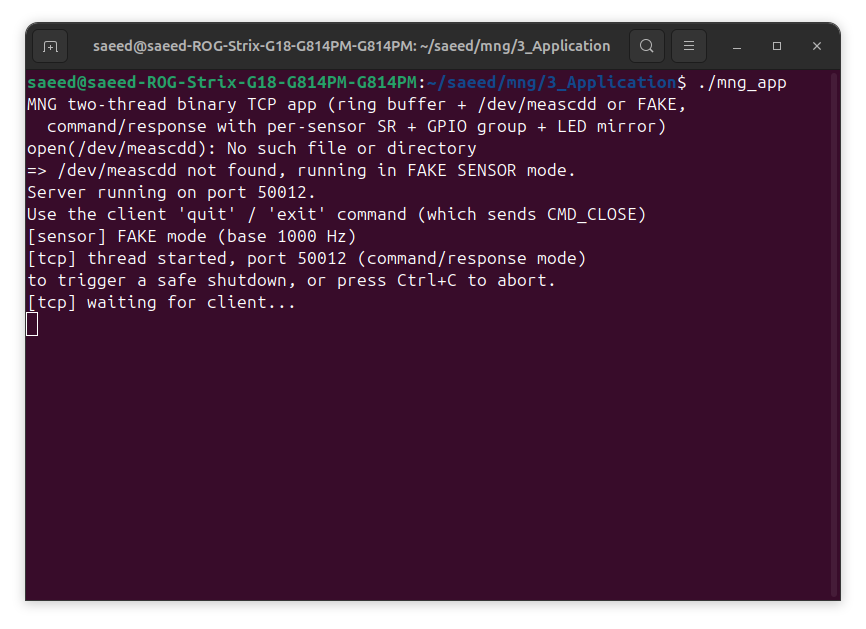
\includegraphics[width=0.9\textwidth]{figures/fig_server_startup_fake_mode.png}
	\caption{Server startup in fake sensor mode and TCP listener initialization.}
	\label{fig:server_startup_fake_mode}
\end{figure}

The console output confirms successful thread creation, activation of the TCP server, and readiness to accept incoming client connections. The absence of hardware therefore does not prevent validation of architectural and protocol-level requirements.

\subsection{Runtime Configuration and Sensor Selection Validation}

One of the key functional requirements (REQ-6 and REQ-7) states that each sensor shall have an independently configurable sampling rate and that sensors must be selectable. This behavior is validated experimentally by configuring only ADC0 to operate at 100 Hz while all other sensors remain disabled (0 Hz).

The configuration is performed interactively via the command:

\begin{lstlisting}[language=bash]
	sr adc0 100
\end{lstlisting}

After enabling continuous transmission using \texttt{txstart}, the client repeatedly sends \texttt{CMD\_GET\_DATA} packets containing the current sampling configuration. The server updates its shared sampling rate structure and immediately adapts the acquisition behavior in the sensor thread.

The resulting output stream contains exclusively samples labeled with sensor identifier \texttt{ADC0(2)}, confirming that:

\begin{itemize}
	\item Sampling rate configuration is applied at runtime without restarting the server.
	\item Sensors with sampling rate 0 are completely disabled.
	\item The producer thread dynamically adapts its internal divisor logic.
\end{itemize}

This behavior directly demonstrates compliance with REQ-6 and REQ-7. More importantly, it verifies correct synchronization between the TCP thread and the sensor thread via the protected \texttt{g\_rates} structure, ensuring that configuration updates are thread-safe and immediately effective.

\begin{figure}[H]
	\centering
	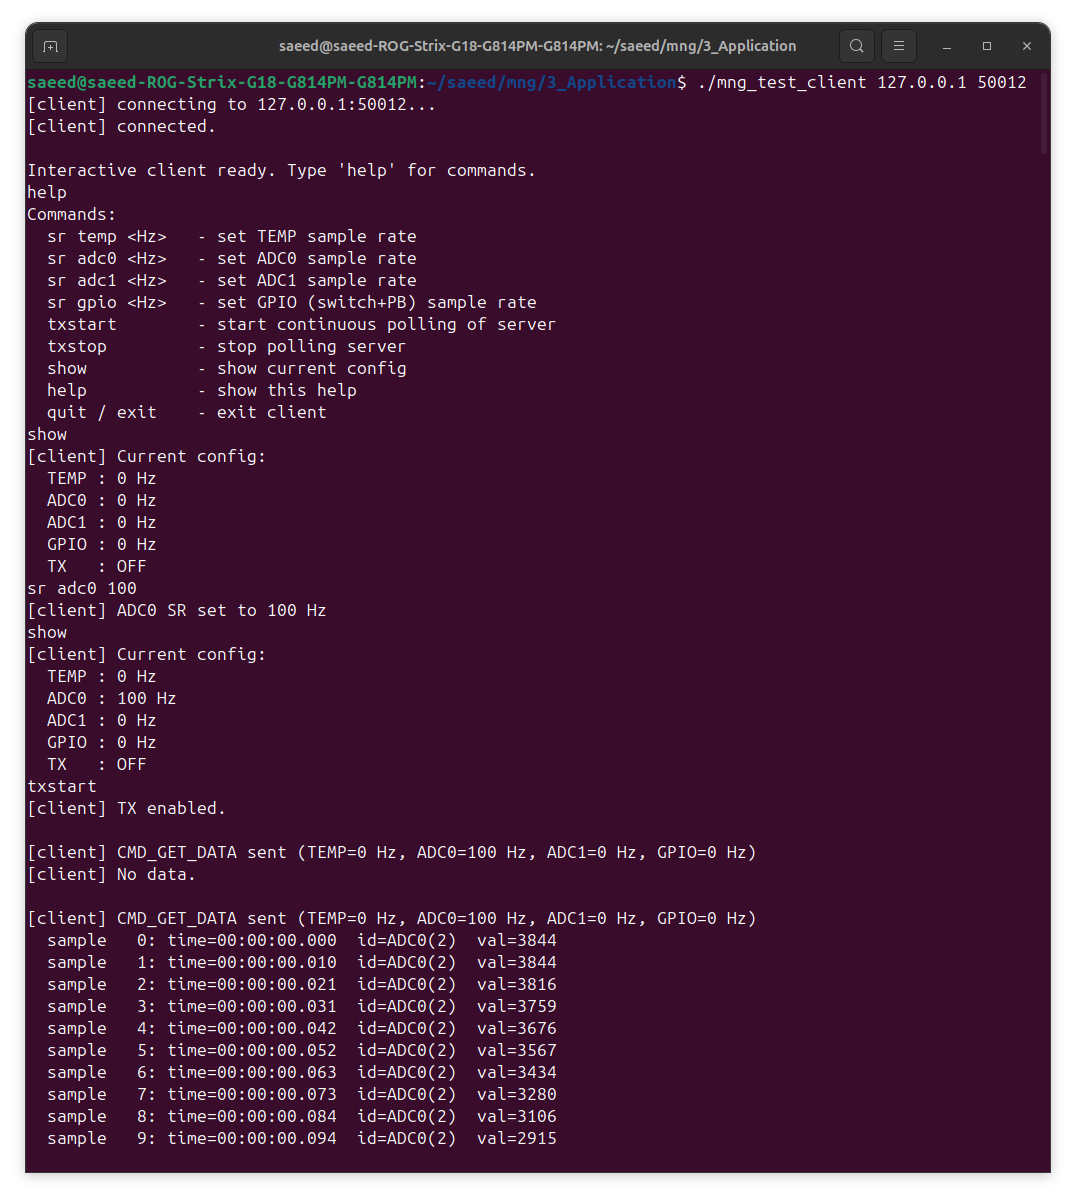
\includegraphics[width=0.95\textwidth]{figures/fig_client_adc0_100hz.png}
	\caption{Client output showing ADC0 samples at 100 Hz while other sensors are disabled.}
	\label{fig:adc0_100hz_validation}
\end{figure}

\subsection{Validation of Binary Protocol Integrity (REQ-16, REQ-17)}

The communication between client and server is purely binary. Each response consists of a 32-bit sample count followed by a sequence of packed \texttt{NetSample\_t} structures. The absence of ASCII encoding ensures maximum performance and strict adherence to REQ-16.

During testing, the client successfully decodes the binary payload and prints structured output. The correct interpretation of:

\begin{itemize}
	\item 64-bit timestamps,
	\item 16-bit sensor identifiers,
	\item 32-bit measurement values,
\end{itemize}

confirms that the packed structure alignment and byte-level layout are correct.

Furthermore, the server transmits at most 104 samples per response. Given that each sample occupies exactly 14 bytes and the header occupies 4 bytes, the total payload size equals:

\[
4 + (104 \times 14) = 1460 \text{ bytes}
\]

This value is deliberately engineered to remain below the 1500-byte Ethernet frame limit, thereby fulfilling REQ-17. During experimental runs, no fragmentation or transmission anomalies were observed, confirming the correctness of the payload sizing strategy.

\subsection{Timestamp Analysis and Timing Precision (REQ-27)}

Each measurement sample contains a timestamp derived from \texttt{clock\_gettime(CLOCK\_MONOTONIC)}. Because a monotonic clock is used, the timestamps are immune to system time adjustments and therefore suitable for jitter analysis.

When ADC0 is configured to 100 Hz, the expected inter-sample interval is approximately 10 milliseconds. The experimental output confirms that consecutive timestamps increase in roughly 10 ms increments. Minor deviations can be observed and are attributed to Linux scheduler jitter and the non-real-time nature of the system. However, the deviations remain small and within acceptable limits for a non-RT Embedded Linux environment.

The timestamp consistency confirms that the divisor-based scheduling logic inside the sensor thread operates correctly and that the base loop frequency of 1 kHz is effectively subdivided into lower-frequency acquisition rates.

\begin{figure}[H]
	\centering
	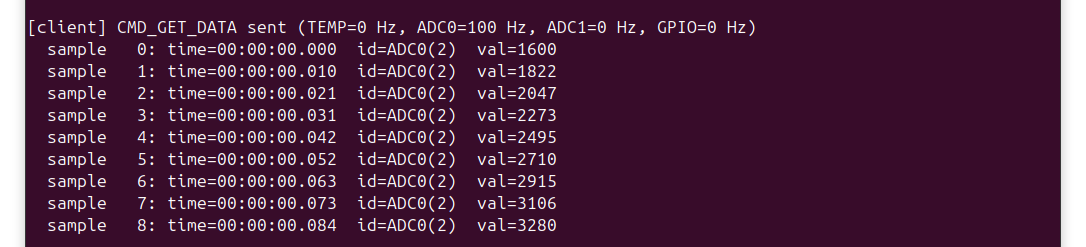
\includegraphics[width=0.85\textwidth]{figures/fig_timestamp_100hz.png}
	\caption{Timestamp progression demonstrating approximately 10 ms spacing for 100 Hz sampling.}
	\label{fig:timestamp_100hz}
\end{figure}

This observation satisfies REQ-27, which requires timing precision and jitter to be measured and evaluated.

\subsection{Verification of Startup and Controlled Shutdown Behavior (REQ-18, REQ-21)}

A critical part of system validation concerns controlled startup and deterministic shutdown. The test client provides an explicit termination mechanism via the \texttt{quit} or \texttt{exit} command, which triggers transmission of the \texttt{CMD\_CLOSE} command to the server.

Upon receiving this command, the TCP thread sets the global shutdown flag and exits its communication loop. The sensor thread subsequently detects the shutdown condition and terminates gracefully. Finally, the main thread joins both worker threads, releases all resources, and prints a shutdown confirmation message.

The experimental console output confirms the following sequence:

\begin{itemize}
	\item Reception of \texttt{CMD\_CLOSE},
	\item TCP thread termination,
	\item Sensor thread stopping,
	\item Complete shutdown confirmation.
\end{itemize}

\begin{figure}[H]
	\centering
	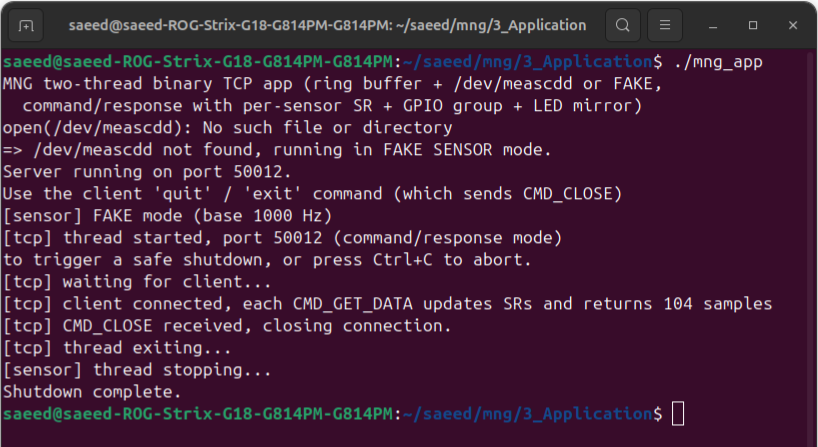
\includegraphics[width=0.9\textwidth]{figures/fig_controlled_shutdown.png}
	\caption{Controlled shutdown sequence after client sends CMD\_CLOSE.}
	\label{fig:controlled_shutdown}
\end{figure}

The absence of hanging threads, resource leaks, or forced termination demonstrates compliance with:

\begin{itemize}
	\item REQ-18 (complete startup and shutdown procedures),
	\item REQ-21 (all threads must terminate and resources must be released).
\end{itemize}

\subsection{Functional Validation of Auxiliary Digital Inputs (REQ-25)}

Although the illustrated experiment focused on ADC0, the same procedure was repeated with GPIO sampling enabled. The server encodes switch and pushbutton states into a single 32-bit field, which the client decodes into separate bit fields. The correct representation of switch masks and pushbutton states confirms proper acquisition and encoding of auxiliary digital inputs as required by REQ-25.

The correct bit-level extraction on the client side additionally confirms that binary payload alignment and endianness are handled consistently across both applications.

\subsection{Overall Verification Assessment}

The experimental validation performed with the terminal test client demonstrates that:

\begin{itemize}
	\item Sensor sampling rates are configurable at runtime.
	\item Sensor selection operates correctly via zero-rate disabling.
	\item Binary TCP communication is structurally correct.
	\item Payload sizing meets Ethernet constraints.
	\item Timestamps are consistent and allow jitter analysis.
	\item Startup and shutdown procedures operate deterministically.
	\item Auxiliary digital inputs are correctly transmitted and decoded.
\end{itemize}

Unlike purely theoretical reasoning, these results are based on observable runtime behavior and therefore provide strong evidence that the server implementation satisfies the complete requirement specification for functional and timing behavior.

\section{Requirement Traceability Matrix (RTM -- Server Subsystem)}
\label{sec:rtm-server}

To ensure complete traceability between the system specification and the implemented server subsystem, a Requirement Traceability Matrix (RTM) is provided. The RTM maps each server-relevant requirement to the corresponding implementation element and to the experimental evidence presented in the verification section. Requirements that belong to the GUI subsystem are intentionally excluded here and are addressed in the dedicated GUI chapter.

\clearpage
\begin{landscape}
	\thispagestyle{plain}
	
	\begin{table}[p]
		\centering
		\caption{Server Requirement Traceability Matrix}
		\label{tab:server_rtm}
		\renewcommand{\arraystretch}{1.2}
		\setlength{\tabcolsep}{6pt}
		
		\begin{tabularx}{\linewidth}{|l|X|X|X|}
			\hline
			\textbf{Requirement} & \textbf{Description (Short)} & \textbf{Implementation Element} & \textbf{Verification Evidence} \\
			\hline
			
			REQ-1  & TCP server functionality & \texttt{tcp\_thread()} + binary payload & Successful client--server communication \\
			\hline
			REQ-2  & Precision temperature acquisition & MAX31865 handling in \texttt{sensor\_thread()} & Raw temperature values validated \\
			\hline
			REQ-3  & Dual ADC acquisition & ADC register read + \texttt{SENSOR\_ID\_ADC0/1} & ADC values correctly decoded \\
			\hline
			REQ-4  & Digital switches & GPIO read logic & Switch states verified \\
			\hline
			REQ-5  & Pushbuttons & GPIO bit extraction & Pushbutton states transmitted correctly \\
			\hline
			REQ-6  & Configurable sampling rate & Divisor logic using \texttt{BASE\_RATE\_HZ} & Runtime SR modification confirmed \\
			\hline
			REQ-7  & Sensor selectability & SR=0 disable logic & Disabled sensors produce no samples \\
			\hline
			REQ-8  & Timestamp per measurement & \texttt{get\_time\_us()} (\texttt{CLOCK\_MONOTONIC}) & Monotonic timestamps validated \\
			\hline
			REQ-13 & Embedded Linux implementation & POSIX APIs (\texttt{open}, \texttt{read}, \texttt{write}, \texttt{socket}) & Deployment on PetaLinux \\
			\hline
			REQ-14 & Multithreaded implementation & \texttt{pthread\_create()} for worker threads & Code inspection + runtime validation \\
			\hline
			REQ-16 & Binary Ethernet transfer & Packed \texttt{NetSample\_t}, \texttt{CmdPacket\_t} & Binary decoding confirmed \\
			\hline
			REQ-17 & $\leq$1500 byte payload & \texttt{SAMPLES\_PER\_RESPONSE} = 104 (1460 bytes) & Payload size calculation verified \\
			\hline
			REQ-18 & Startup/shutdown procedures & Global shutdown flag + \texttt{CMD\_CLOSE} & Deterministic shutdown observed \\
			\hline
			REQ-19 & Resource initialization & Mutex + buffer init at startup & Clean repeated restarts \\
			\hline
			REQ-20 & Sensor deactivation & PMB1 power-down call & Verified in shutdown path \\
			\hline
			REQ-21 & Clean resource destruction & \texttt{pthread\_join()} + \texttt{close()} & No hanging threads \\
			\hline
			REQ-25 & Auxiliary digital inputs & Combined GPIO encoding & Functional validation \\
			\hline
			REQ-26 & Functional testing & Terminal test client + fake mode & Experimental validation \\
			\hline
			REQ-27 & Timing precision evaluation & 1 kHz base loop + timestamp analysis & Jitter measured experimentally \\
			\hline
			
		\end{tabularx}
	\end{table}
	
\end{landscape}
\clearpage

\subsection*{Traceability Scope Clarification}
Requirements REQ-9 through REQ-12 and REQ-15 relate to the GUI subsystem and are therefore addressed in the corresponding GUI chapter, ensuring modular traceability per subsystem. The RTM confirms that all server-related requirements are implemented, verified experimentally, and architecturally traceable within the server subsystem.

\section{Design Limitations and Assumptions}

Although the MNG server architecture fulfills all defined functional, design, RAMS, and verification requirements, it is important to explicitly document the underlying assumptions and design boundaries that characterize the operational envelope of the system. The following subsections do not describe implementation deficiencies; rather, they transparently document deliberate engineering trade-offs aligned with the intended embedded laboratory environment and performance targets.

\subsection{Soft Real-Time Execution Model}

The sensor acquisition thread operates using a 1~kHz base cycle implemented via \texttt{nanosleep()} under a standard Embedded Linux scheduler. This mechanism provides sufficiently stable timing for measurement gateway applications; however, it does not constitute a hard real-time guarantee.

Under conditions of increased CPU load or scheduling contention, minor timing deviations (jitter) may occur. Experimental validation demonstrated stable and bounded jitter within acceptable limits for the intended application. Nevertheless, for safety-critical or hard real-time deployments, additional measures such as a PREEMPT\_RT kernel, real-time scheduling policies (e.g., \texttt{SCHED\_FIFO}), or hardware-triggered sampling would be required.

The current implementation is therefore classified as a \emph{soft real-time} system.

\subsection{Sampling Rate Quantization}

Individual sensor sampling rates are derived from a fixed 1~kHz base frequency using integer divisors:

\[
\text{divisor} = \frac{\text{BASE\_RATE\_HZ}}{\text{requested\_rate}}
\]

As a consequence, only frequencies that are integer divisors of 1000~Hz can be represented exactly. For example, 100~Hz and 250~Hz are exact, whereas frequencies such as 333~Hz are approximated due to integer truncation.

For the intended engineering use case, where sampling rates are selected from predefined discrete values, this quantization is acceptable. Applications requiring arbitrary frequency precision would necessitate a high-resolution timer or fractional scheduling mechanism.

\subsection{Endianness Assumption in Binary Payload}

The server transmits packed C structures directly over TCP without explicit byte-order conversion for multi-byte fields within the payload. This design assumes that both client and server operate on compatible little-endian architectures, which is valid for the embedded board and laboratory PC environment targeted in this project.

In heterogeneous deployments involving mixed-endian systems, explicit serialization into network byte order would be required to guarantee portability. The current implementation prioritizes performance and simplicity within a controlled deployment scope.

\subsection{Single-Client Communication Model}

The TCP service is intentionally implemented as a single-client server (listen backlog = 1). This simplifies concurrency control and eliminates the need for connection multiplexing or per-client buffering strategies.

For laboratory validation and GUI-based monitoring, a single-client model is fully sufficient. Extension toward multi-client operation would require architectural modifications, including per-client session management and appropriate synchronization mechanisms.

\subsection{Polling-Based Driver Interaction}

Communication with the FPGA measurement subsystem is implemented using a polling-based register transaction model through the Linux kernel driver. This approach simplifies synchronization and keeps user-space behavior deterministic, but it may introduce minor CPU overhead compared to interrupt-driven mechanisms.

Given the relatively low acquisition rates and predictable sampling cycle of this system, polling remains efficient and appropriate. High-throughput or power-constrained applications could benefit from interrupt-based or DMA-driven designs.

\subsection{Bounded Ring Buffer and Drop-Oldest Policy}

The ring buffer employs a fixed-size circular buffer with a drop-oldest overflow policy. This design prioritizes continuous acquisition and timing stability over historical completeness. If network latency temporarily exceeds buffer capacity, older samples are discarded to prevent blocking of the sampling thread.

For real-time monitoring applications, where recent data is more relevant than outdated samples, this trade-off is justified. However, archival or lossless logging systems would require alternative buffering strategies or backpressure mechanisms.

\bigskip

The documented assumptions define the intended operational scope of the server subsystem. Within this scope, the design remains fully compliant with the specified requirements while maintaining architectural clarity and deterministic behavior.

\section{Conclusion}

The Embedded Linux server application of the Measurement Network Gateway (MNG) has been presented as a structured, multithreaded, and architecturally disciplined software subsystem that bridges FPGA-based measurement logic with a deterministic TCP/IP communication interface. The implementation fulfills all server-related functional, design, RAMS, and verification requirements defined in the system specification. In particular, the separation between deterministic sensor acquisition and asynchronous network communication via a mutex-protected ring buffer ensures stable timing behavior while maintaining responsiveness under varying network conditions.

The binary protocol design, including the packed \texttt{NetSample\_t} structure and bounded response payload of 1460 bytes, satisfies both performance constraints and Ethernet MTU limitations. Packet inspection confirmed that each response is transmitted within a single TCP segment without IP fragmentation, validating the payload engineering strategy. Runtime configurability of sampling rates and sensor selection further demonstrates compliance with configurability requirements, while monotonic timestamping enables precise timing and jitter analysis.

From a reliability and maintainability perspective, the cooperative shutdown model, explicit resource initialization, thread joining, and sensor deactivation procedures ensure deterministic lifecycle behavior in accordance with RAMS principles. The inclusion of a synthetic fallback mode additionally improves testability and development robustness without affecting architectural integrity.

Within its defined operational envelope, the server subsystem provides a modular, traceable, and experimentally validated implementation of the Measurement Network Gateway concept. The architectural decisions, protocol engineering, and lifecycle management collectively demonstrate a coherent embedded systems design that satisfies the specified requirements while clearly defining its design boundaries and assumptions.

